\documentclass[9pt]{beamer}

% Created By Gouthaman KG

\usepackage[utf8]{inputenc}
\usepackage[T1]{fontenc}
\usepackage{listings}


\definecolor{codegreen}{rgb}{0,0.6,0}
\definecolor{codegray}{rgb}{0.5,0.5,0.5}
\definecolor{codepurple}{rgb}{0.58,0,0.82}
\definecolor{backcolour}{rgb}{0.95,0.95,0.92}
\lstdefinestyle{mystyle}{
    backgroundcolor=\color{backcolour},   
    commentstyle=\color{codegreen},
    keywordstyle=\color{magenta},
    numberstyle=\tiny\color{codegray},
    stringstyle=\color{codepurple},
    basicstyle=\ttfamily\footnotesize,
    breakatwhitespace=false,         
    breaklines=true,                 
    captionpos=b,                    
    keepspaces=true,                 
    numbers=left,                    
    numbersep=5pt,                  
    showspaces=false,                
    showstringspaces=false,
    showtabs=false,                  
    tabsize=2
}

\lstset{style=mystyle}
\usepackage{styles/fluxmacros}
\usefolder{styles}
\usetheme[style=asphalt]{flux}
\usepackage{booktabs}
\usepackage{colortbl}
\usepackage{ragged2e}
\usepackage{schemabloc}
\usepackage{hyperref}
\usepackage{amsfonts}
\usepackage{amssymb}
\usepackage{amsthm}
\usepackage{amsmath}
\usepackage{amsopn} 
\usepackage{amsmath, amstext}
\usebackgroundtemplate{

\includegraphics[width=\paperwidth,height=\paperheight]{assets/background.jpg}}
\title{Generator liczb losowych}
\subtitle{Projekt na przedmot}
\subtitle{Rachunek Prawdopodobieństa i Statystyka}
\author{Paweł Pyciński}
\institute{Uniwersytet Jagielloński}
\titlegraphic{assets/uj3.jpg}

\begin{document}

% Generate title page
\titlepage

\begin{frame}

 \frametitle{TABLE OF CONTENTS}
 \tableofcontents
\end{frame}

\section{Wprowadzenie}
\begin{frame}
  \frametitle{Cel Projektu}
  Celem projektu jest stworzenie generatora całkowitych liczb pseudolosowych o rozkładzie równomiernym. Na podstawie stworzonego generatora należy stworzyć generatory o rozkładzie jednostajnym (na przedziale [0,1]), Bernoulliego, dwumianowego, Poissona, wykładniczego i normalnego. Następnie należy przetestować powstałe generatory.
\end{frame}
\begin{frame}
  \frametitle{Wprowadzenie, opis problemu}
  \begin{block}{Definicja}
    \textbf{Generator liczb pseudolosowych} – program lub podprogram, który na podstawie niewielkiej ilości informacji generuje deterministycznie ciąg bitów, który pod pewnymi względami jest nieodróżnialny od ciągu uzyskanego z prawdziwie losowego źródła.
    \end{block}

  Generator liczb pseudolosowych nie bez powodu jest \textbf{pseudolosowy}, problem z otrzymaniem liczb losowych wynika z deterministycznego charakteru komputera i wykonywanych przez niego operacji. Gdy człowiek dokonuje rzutu kością, nie wie co wypadnie. Taka sama operacja na komputerze wymaga działania, którego wynik jest nieprzewidywalny – żadna z operacji wykonywanych przez procesor nie posiada takiej cechy.

  Problem starano się rozwiązać wykorzystując zewnętrzne źródła sygnałów losowych (np. generatory białego szumu ), jednakże w tego typu urządzenia nie są standardowo wyposażano komputery osobiste. Próbowano także wykorzystać szumy kart dźwiękowych, jednakże system ten nie rozpowszechnił się z prostej przyczyny – różne karty dźwiękowe szumią różnie, a te z górnej półki nie szumią prawie wcale.
\end{frame}
\section{Sposoby generowania liczb pseudolosowych}
\begin{frame}
  \frametitle{Sposoby generowania liczb pseudolosowych}
  Jest wiele sposobów generowania liczb pseudolosowych. Jedną z grup generatorów są generatory liniowe. tworzą ciąg liczb według schematu:
  \begin{equation*}
    X_{n+1}= (a_1X_n+a_2X_{n-1}+\ldots+a_kX_{n-k+1}+c)mod(m)
  \end{equation*}
  gdzie $a_1$,\ldots,$a_k$, $c$, $m$ -parametry generatora (ustalone liczby)

  Generatory używające operacji modulo nazywamy \textbf{kongruencyjnymi}. Każdy kolejny wyraz (liczba pseudolosowa) w generatorze liniowym to suma pewnych poprzednich wyrazów pomnożonych każdy z każdą o jakiś skalar i brane z nich jest modulo. 
  
  Generator mulitplikatywny tworzy liczby według schmatu:
  \begin{equation*}
    X_{i+1}=(aX_{i}+c)mod(m) \iff c=0
  \end{equation*}
Kolejny wyraz tworzymy po przez pomnożenie poprzedniego przez jakiś skalar. Gdy $c \neq  0$ to generator jest kongurentnie mieszany.
\end{frame}
\section{Własny generator}
\begin{frame}
  \frametitle{Własny generator}
    Swój generator postanowiłem zbudować na bazie generatora mulitplikatywnego. Jest to jeden z łatwiejszych generatorów, prosty do implementacji. 
    
    Posiada on niestety dwie poważne wady:
    \begin{enumerate}
      \item Gererator generuje liczby ciągu w sposób deterministyczny przez co łatwo jest wyliczyć kolejną liczbę.
      \item Wybierając złe czynniki możemy spowodować, że okres generatora będzie mały przez co będzie działał niepoprawnie lub będzie generował bardzo mało liczb losowych.
      \item Generowane liczby lokalizują się na hiperpłaszczyznach, których położenie uzależnione jest od parametrów generatora.
    \end{enumerate} 
    \begin{figure}[h]
      \begin{center}
      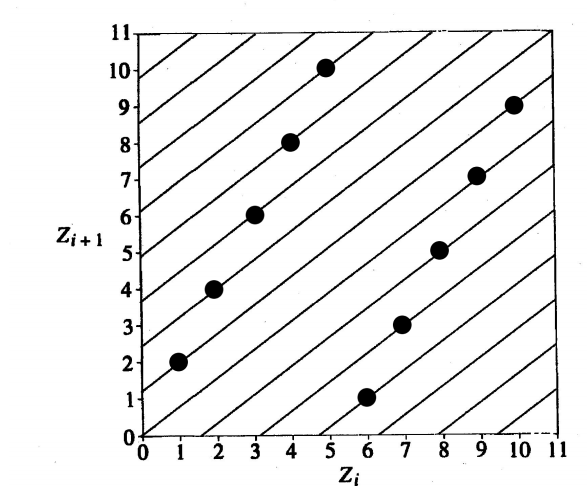
\includegraphics[width=0.2\textwidth]{assets/1.PNG}
      \end{center}
      \end{figure}
    Przez wyżej wymienione czynniki nie może być on stosowany w kryptografii.
\end{frame}
\begin{frame}
  \frametitle{Własny generator}
  Przed zaimplementowaniem pozostał jeszcze wybór $m$ oraz $a$ dla naszego generatora.

  Niech $m=2^{32}$, jest to liczba o 1 większa od zakresu unsigned int'a, dzięki czemu nasza kongruencja potencjalnie będzie mogła zwracać wszyskie liczby które jesteśmy w stanie zapisać na 4 bajtach float'a w większości języków programowania. Ponadto niech $a=747796405.$
  \begin{figure}[h]
    \begin{center}
    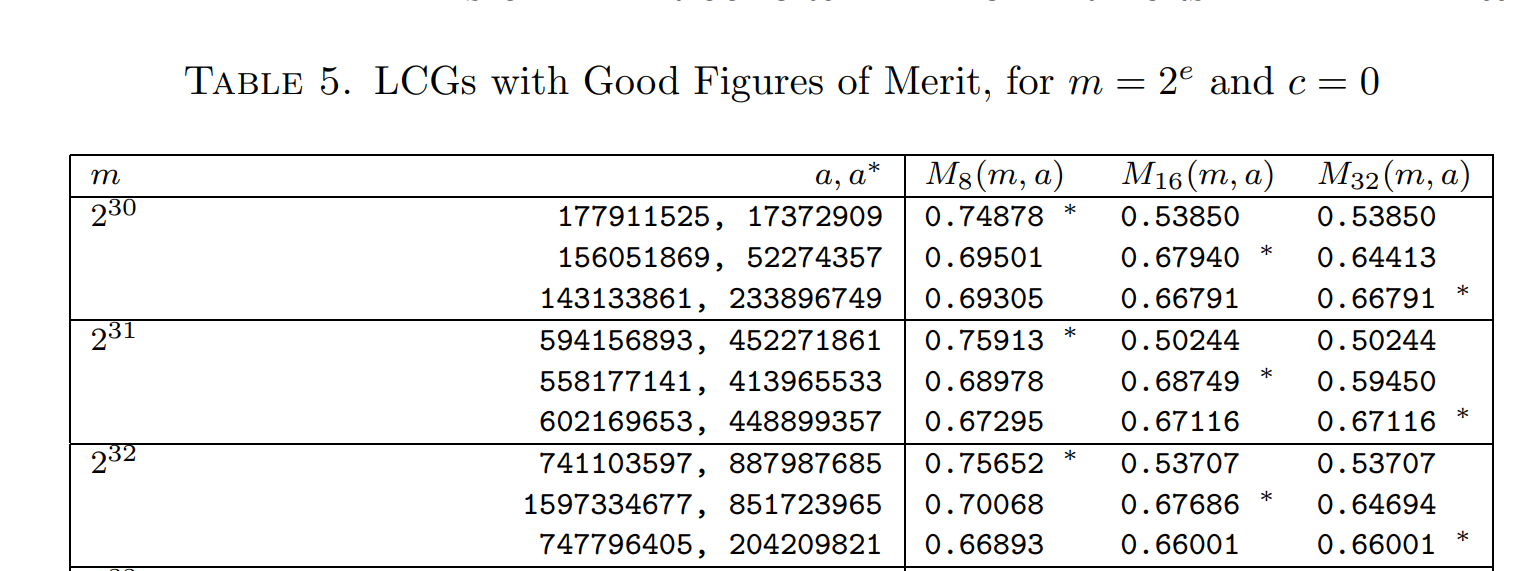
\includegraphics[width=0.7\textwidth]{assets/table.PNG}
    \end{center}
    \end{figure}
\end{frame}
\section{Własny generator - kod źródłowy}
 \begin{frame}[containsverbatim]
  \frametitle{Własny generator - kod źródłowy}
   \begin{lstlisting}[language=Python, caption=Klasa generatora]
    class generator:

        def __init__(self, seed):
            self.value = seed
            self.a = 747796405
            self.m = 4294967296

        def generateRandom(self):
            self.value = (self.a*self.value) % self.m
            return self.value
    \end{lstlisting}
    Klasa generatora posiada konstruktor który jako argument przyjmuje ziarno czyli dowoloną liczbę początkową która rozpocznie budowanie pseudolosowy ciąg. Jest także metoda która zwaraca kolejną wygenerowaną liczbę.
\end{frame}
\section{Modyfikacje generatora dla uzyskania zadanych rozkładów}
\begin{frame}[containsverbatim]
  \frametitle{Rozkład jednostajny}
  Aby uzyskać liczby z rozkładu jednostajnego na przedziale $[0,1]$ wystarczy podzielić przez ustalone wcześniej $m=4294967296$, zauważmy że po takiej operacji największą liczbą możliwą do uzyskania będzie 1, natomiast pozostałe liczby będą należały to przedziału $[0,1]$.
  \begin{lstlisting}[language=Python, caption=Metoda rozkładu jednostajnego]
    def uniformDistribution(self):
        return self.generateRandom()/self.m
    \end{lstlisting}
\end{frame}
\begin{frame}[containsverbatim]
  
  \frametitle{Rozkład Bernoulliego}
  Rozkład Bernoulliego, jest rozkładem dwupunktowym, aby uzyskać ten rozkład skorzystam z metody którą przygotowałem dla rozkładu jednostajnego. Ustalmy dowolne $P\in [0,1]$. Jeśli wylosowana liczba przez metodę rozkładu jednostajnego będzie mniejsza od p to zwrócimy 0, w przeciwnym razie 1.
  \begin{lstlisting}[language=Python, caption=Metoda rozkładu Bernoulliego]
    def bernoulliDistribution(self, probability):
        rand = self.uniformDistribution()
        if ( rand<= probability):
            return 0
        else:
            return 1
    \end{lstlisting}
\end{frame}
\begin{frame}[containsverbatim]
  \frametitle{Rozkład Dwumianowy}
  Rozkład dwumianowy jest to liczba sukcesów w $n$ próbach Bernoulliego. W implementacji wykorzystałem wcześniej przygotowaną metodę generowania próby Bernoulliego, wywołanie jej $samples$ razy daje nam rozkład Dwumianowy
  \begin{lstlisting}[language=Python, caption=Metoda rozkładu Dwumianowego]
    def binomialDistribution(self,probablity, n):
        counter = 0
        for i in range(n):
            counter+=self.bernoulliDistribution(probablity)
        return counter
    \end{lstlisting}
\end{frame}
\begin{frame}[containsverbatim]
  \frametitle{Rozkład Poissona}
  Rozkład Poissona modeluje zdarzenia rzadkie. Jest on parameryzowany zmienną $\lambda$ która jest równa oczekiwanej liczbie zdarzeń w danym przedziale czasu. Jest wiele algorytmów generujących ten rozkład na potrzeby naszego generatora wystaczy zastosować najprostszy z nich czyli \textbf{ Algorytm Knutha}
  \begin{lstlisting}[language=Python, caption=Metoda rozkładu Poissona]
    def poissonDistribution(self, lambdapoiss):
        limit = math.exp(-lambdapoiss)
        n = 0
        p = self.uniformDistribution()
        while(p>=limit):
            n+=1
            p*=self.uniformDistribution()
        return n
    \end{lstlisting}
\end{frame}
\begin{frame}
  \frametitle{Rozkład Wykładniczy, wprowadzenie}
  Rozkład wykładniczy modeluje czas między kolejnymi zdarzeniami, jeśli w jednostce czasu zachodzi średnio $\lambda$ niezależnych zdarzeń. 
  
  Metodę generującą rozkład wykładniczy możemy uzyskać stosując metodę odwórconej dystrybuanty. Dystrybuanta określonego rozkładu prawdopodobieństwa jest funkcją $F: \mathbb{R} \rightarrow \mathbb{R} $ niemalejąca i prawostronnie ciągła Dystrybuanta jednoznacznie definiuje rozkład prawdopodobieństwa i ma następujący związek z gęstością prawdopodobieństwa: $ F(x) =\int_{x}^{-\infty}  f(y) \,dy $. Jeśli uda się znaleźć $F^{-1}$ to $U=F(x) \rightarrow x=F^{-1}(U)$ zmienna losowa $x$ ma rozkład o dystrybuancie $F$, $U$ jest zmienną losową o rozkładzie jednostajnym. Krótki dowód dlaczego tak jest:

  Niech $X=F^{-1}(U)$ zmienna losowa
  \begin{gather*}
    P \{X\leq x\} = P\{F^{-1}(U)\leq x\} \\
    = P\{U\leq F(x)\} \\
    =F(x)
  \end{gather*}
\end{frame}
\begin{frame}[containsverbatim]
  \frametitle{Rozkład Wykładniczy}
  Przejdźmy teraz do rozkładu wykładniczego. Jego gęstość prawdopodobieństwa dana jest wzorem:
  \begin{equation*}
    f(x)=e^{-x},x\in [0,\infty)
  \end{equation*}
  Natomiast dystrybuanta jest całką z funkcji gęstości.
  \begin{gather*}
    F(x)=\int_{x}^{0}  e^{-x}\,dx =1-e^{-x} \\
    F(x)=1-e^{-x}=U \\
    e^{-x}=1-U \\
    F^{-1}(x)=x=-\ln(1-U) \\
    U \in (0,1) \rightarrow x\in (0, \infty)
  \end{gather*}
  \begin{lstlisting}[language=Python, caption=Metoda rozkładu Poissona]
    def exponentialDistribution(self):
        return -math.log(1-self.uniformDistribution())
    \end{lstlisting}
\end{frame}
\begin{frame}
  \frametitle{Rozkład normalny}
  Rozkład normalny jest jednym z najważniejszych rozkładów prawdopodobieństwa, odgrywający ważną rolę w statystyce. Przyczyną jego znaczenia jest częstość występowania w naturze. Jeśli jakaś wielkość jest sumą lub średnią bardzo wielu drobnych losowych czynników, to niezależnie od rozkładu każdego z tych czynników jej rozkład będzie zbliżony do normalnego (na podstawie CTG).

  Jest wiele algorytmów aby uzyskać rozkład normalny. Ja w swojej implementacji zastosowałem polarny algorytm Boxa-Mullera nazwywany inaczej sposobem polarnym.
  Polega on na wylosowaniu dwóch zmiennych $(x,y)$ z przedziału $(-1,1)$ tak aby $0<x^2+y^2<1$ a następnie należy podstawić do wzoru:
  \begin{equation*}
    x\sqrt{\frac{-2\ln{s}}{s}} \:\: \:  lub \:\: \:  y\sqrt{\frac{-2\ln{s}}{s}}
  \end{equation*}
  wzory te stosujemy na zmianę dlatego przyda się drobna modyfikacja obecnego genereatora o dodanie nowej zmiennej którą będziemy zmieniać w zależności o zastosowanego wzoru.
\end{frame}
\begin{frame} [containsverbatim]
  \frametitle{Rozkład normalny - kod źródłowy}
  \begin{lstlisting}[language=Python, caption=Metoda rozkładu normalnego]
    def normalDistribution(self):
    if(self.whichOne == 1):
        self.whichOne = 0
        return self.prevValue
    else:
        x = self.uniformDistribution()*2-1
        y=self.uniformDistribution()*2-1
        s=x*x+y*y
        while (s>=1 or s==0):
            x = self.uniformDistribution()*2-1
            y=self.uniformDistribution()*2-1
            s=x*x+y*y
        s=math.sqrt((math.log(s)*(-2))/s)
        self.prevValue=y*s
        self.whichOne=1
    return x*s 
  \end{lstlisting}
\end{frame}
\section{Test poprawności generatora}
\begin{frame}
  \frametitle{Test poprawności generatora - wprowadzenie}
  Kolejnym etapem jest przetestowanie napisanego wcześniej generatora oraz sprawdzenie czy otrzymane wyniki są zgodne z oczekiwanymi. Do tego celu wykorzystam test $\chi^2$
  \begin{block}{Definicja}
    \textbf{Test chi-kwadrat} – każdy test statystyczny, w którym statystyka testowa ma rozkład chi kwadrat, jeśli teoretyczna zależność jest prawdziwa. Test chi-kwadrat służy sprawdzaniu hipotez. Innymi słowy wartość testu oceniana jest za pomocą rozkładu chi kwadrat. Test najczęściej wykorzystywany w praktyce. Można go wykorzystywać do badania zgodności zarówno cech mierzalnych, jak i niemierzalnych.
    \end{block}
\end{frame}
\begin{frame}
  \frametitle{Test poprawności generatora - omówienie warunków}
  \textbf{Teza zerowa:} Otrzymany rozkład jest pożądanym rozkładem \newline
  \textbf{Teza alternatywna:} Otrzymany rozkład nie jest oczekiwanym rozkładem. \newline
  Należy ukształtować dane w taki sposób aby każda próbka miała co najmniej 5 elementów, przyjmijmy także powszechnie stosowany 5\% stopień akceptacji.
\end{frame}
\begin{frame}
  \frametitle{Generator rozkładu jednostajnego}
  
\end{frame}
\section{Sources}
\begin{frame}
  \frametitle{Sources}
  \begin{itemize}
    \item \url{http://home.agh.edu.pl/~chwiej/mn/generatory_16.pdf}
    \item \url{https://pl.wikipedia.org/wiki/Generator_liczb_pseudolosowych}
    \item \url{https://eduinf.waw.pl/inf/alg/001_search/0022.php}
    \item \url{https://www.ams.org/journals/mcom/1999-68-225/S0025-5718-99-00996-5/S0025-5718-99-00996-5.pdf}
    \item \url{http://staff.iiar.pwr.wroc.pl/grzegorz.mzyk/kmi/kmi03.pdf}
    \item \url{https://math.stackexchange.com/questions/785188/simple-algorithm-for-generating-poisson-distribution/785200}
    \item \url{https://pl.wikipedia.org/wiki/Rozkład_wykładniczy}
    \item \item \url{https://pl.xcv.wiki/wiki/Marsaglia_polar_method}
  \end{itemize}
\end{frame}
\end{document}